\section{\textit{Pre-Trained Model}}

\textit{Pre-trained model} merupakan model yang sudah dilatih terlebih dahulu pada \textit{dataset} yang berukuran besar sehingga model ini sudah mempunyai pemahaman yang mendasar pada tugas bahasa yang universal. \textit{Pre-trained model} dapat dilatih lebih lanjut terhadap suatu \textit{dataset} spesifik untuk menjalankan tugas bahasa yang spesifik juga. Salah satu \textit{pre-trained model} yang menjadi \textit{state-of-the-art} saat ini adalah BERT dan versi bahasa Indonesia-nya yaitu IndoBERT. 

\subsection{\textit{Bidirectional Encoder Representations from Transformers} \\ (BERT)}
\label{sec:bert}

BERT, yang merupakan singkatan dari \textit{Bidirectional Encoder Representations from Transformers}, adalah model \textit{encoder} pemrosesan bahasa alami yang diperkenalkan oleh Google pada tahun 2018 \parencite{bert}. BERT memanfaatkan arsitektur \textit{transformer}, yang telah dibahas sebelumnya, untuk memahami konteks kata dalam teks dengan cara yang lebih mendalam daripada pendekatan sebelumnya. BERT menggunakan pendekatan yang \textit{bidirectional}. BERT mampu memahami teks dari kiri ke kanan atau sebaliknya, BERT memahami konteks kata dengan mempertimbangkan informasi dari kedua arah. Sehingga, model ini memiliki kemampuan untuk pemahaman yang lebih kaya tentang makna dan nuansa dalam teks.

\begin{figure}[ht]
    \vspace{0.25cm}
    \centering
    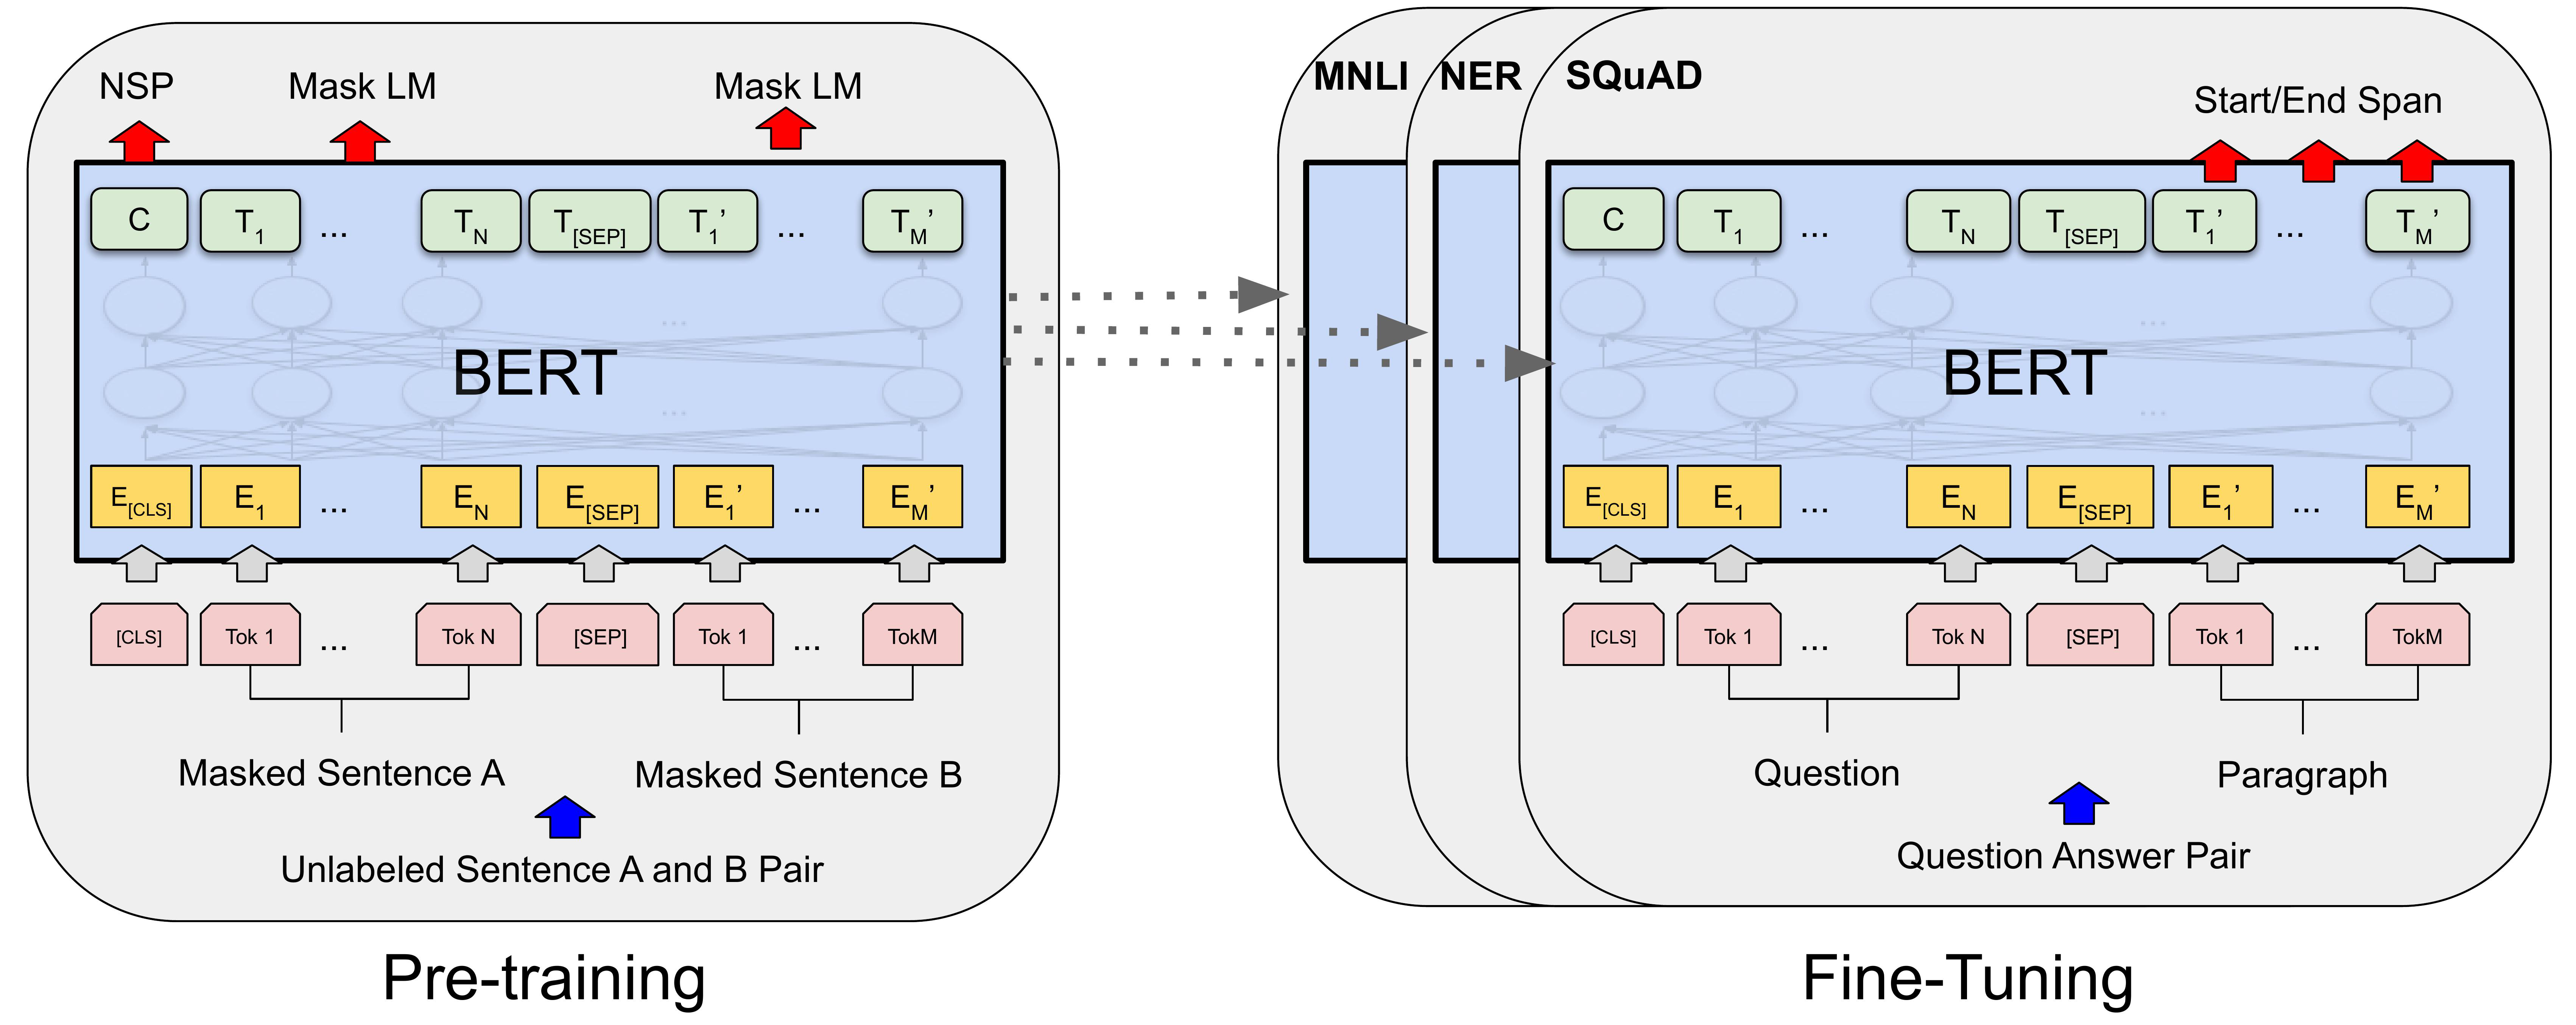
\includegraphics[width=\textwidth]{chapter-2/bert.jpg}
    \caption{Arsitektur BERT \parencite{bert}}
    \label{fig:bert}
\end{figure}

BERT merupakan \textit{pre-trained model} sehingga telah dilatih pada sejumlah besar teks. Data latih BERT diambil dari BooksCorpus dan Wikipedia bahasa Inggris \parencite{bert}. Ini memungkinkan BERT untuk mempunyai pengetahuan mendasar dalam tugas NLP. Ketika digunakan untuk tugas-tugas NLP spesifik, seperti klasifikasi teks atau pemahaman pertanyaan, BERT dapat disesuaikan dengan data tugas spesifik untuk meningkatkan kinerjanya. Seperti yang bisa dilihat pada gambar \ref{fig:bert}, BERT dilatih (\textit{pre-train}) dengan menggunakan dua tugas yaitu \textit{Masked LM} dan \textit{Next Sentence Prediction} (NSP). \textit{Masked LM} melakukan \textit{masking} pada sebagian token dan akan diprediksi oleh model BERT. Sedangkan, untuk NSP, model BERT akan menentukan mana kalimat berikutnya dari kalimat sebelumnya.

Terdapat versi bahasa Indonesia yaitu IndoBERT. IndoBERT merupakan model Transformer yang mirip dengan BERT, namun dilatih dengan bahasa Indonesia \parencite{indolem}. IndoBERT mempunyai konfigurasi yang sama dengan konfigurasi BERT, yaitu 12 \textit{layer} yang masing-masing mempunyai 768 \textit{hidden layer}, 12 \textit{attention head}, dan 3072 \textit{hidden layer} pada \textit{feed-forward layer}. IndoBERT dilatih dengan total 220 juta kata, yang didapatkan dari tiga sumber utama, yaitu Wikipedia Indonesia, sumber berita (Kompas, Tempo, dan Liputan6), dan Indonesian Web Corpus \parencite{indolem}. IndoBERT merupakan \textit{state-of-the-art} pada tugas evaluasi IndoLEM \parencite{indolem}.

\subsection{\textit{Text-to-Text Transfer Transformers} (T5)}

\textit{Text-to-Text Transfer Transformers} atau biasa disebut sebagai T5 merupakan model \textit{encoder decoder} berbasis Transformer. Model ini menggunakan pendekatan \textit{text-to-text} seperti namanya, yang berarti menganggap setiap pemrosesan teks sebagai masukan dan mengeluarkannya sebagai teks juga \parencite{T5}. Dengan pendekatan ini, model T5 dapat digunakan secara langsung pada setiap tugas NLP.

\begin{figure}[ht]
    \vspace{0.25cm}
    \centering
    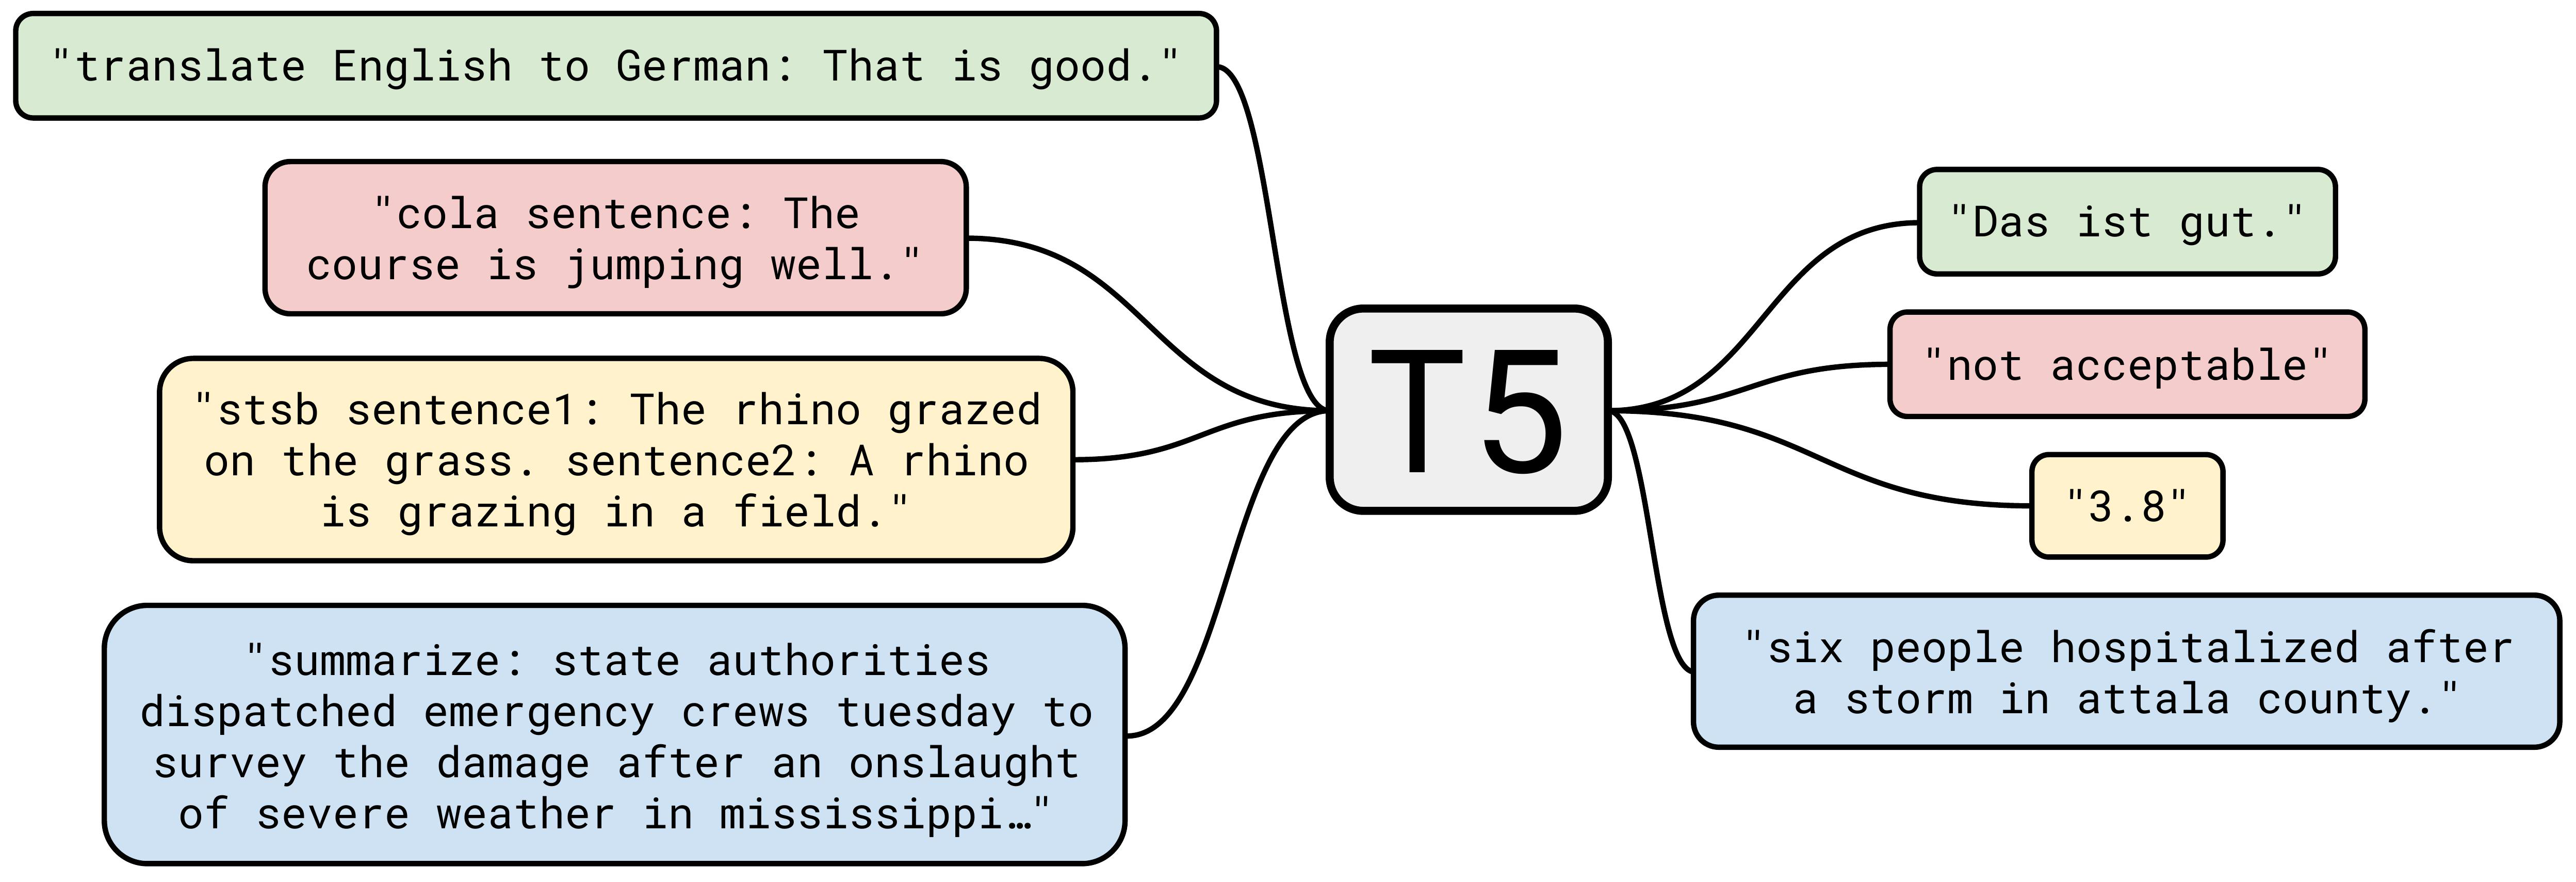
\includegraphics[width=\textwidth]{chapter-2/T5.jpg}
    \caption{\textit{Framework} dari T5 \parencite{T5}}
    \label{fig:T5}
\end{figure}

Pada gambar \ref{fig:T5}, yaitu \textit{framework} dari model T5, setiap tugas pada T5, termasuk \textit{translation, question answering}, dan \textit{classification}, semuanya akan dianggap sebagai masukan teks dan dilatih untuk menghasilkan teks lainnya lagi. T5 dilatih pada dataset \textit{Colossal Cleaned Crawled Corpus} (C4) yang merupakan koleksi dari web publik Common Crawl yang telah dibersihkan.

\begin{figure}[ht]
    \vspace{0.25cm}
    \centering
    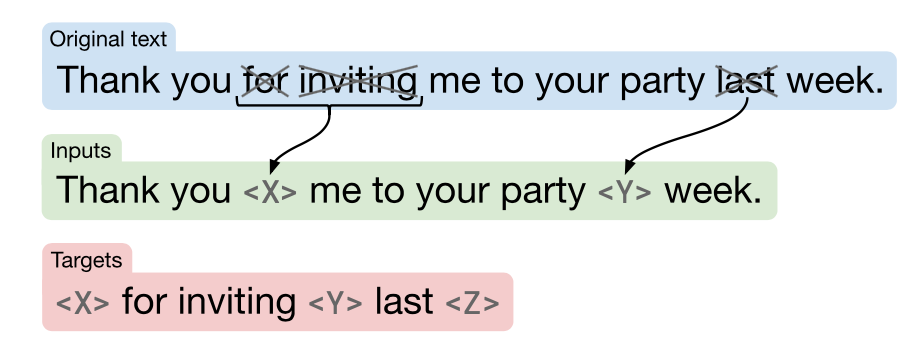
\includegraphics[width=\textwidth]{chapter-2/unsupervised_objective.png}
    \caption{\textit{Unsupervised objectives} dari T5 \parencite{T5}}
    \label{fig:unsupervised-T5}
\end{figure}

Model T5 didesain agar bagian \textit{encoder} dan \textit{decoder}-nya mirip dengan konfigurasi dari BERT \parencite{T5}. Kedua bagian tersebut terdiri dari 12 \textit{layer} yang mempunyai \textit{hidden layer, attention head}, serta \textit{feed-forward}. Mirip dengan MLLM pada BERT, model T5 dilatih \textit{pre-train} dengan menggunakan \textit{unsupervised objectives} yang bisa dilihat pada gambar \ref{fig:unsupervised-T5}. Beberapa kata yang dihilangkan secara konsekutif akan dianggap sebagai satu \textit{sentinel} token yang nantinya akan diprediksi sebagai target oleh T5.

Terdapat versi bahasa Indonesia dari T5, yaitu IndoT5. IndoT5 dilatih secara spesifik untuk bahasa Indonesia dengan menggunakan \textit{framework} pelatihan nanoT5 \parencite{indoT5}. \textit{Dataset} yang digunakan berasal dari CulturaX yang mengandung 23 juta dokumen berbahasa Indonesia. Model IndoT5 menjadi \textit{state-of-the-art} pada tugas \textit{summarization} pada tugas evaluasi IndoLEM \parencite{indoT5}.
